\documentclass[conference]{IEEEtran}
\IEEEoverridecommandlockouts
% The preceding line is only needed to identify funding in the first footnote. If that is unneeded, please comment it out.
\usepackage{cite}
\usepackage{amsmath,amssymb,amsfonts}
\usepackage{algorithmic}
\usepackage{graphicx}
\usepackage{textcomp}
\usepackage{xcolor}
\usepackage{tabularx}
\usepackage{float}
\usepackage{hyperref}
\usepackage{acronym}
\def\BibTeX{{\rm B\kern-.05em{\sc i\kern-.025em b}\kern-.08em
    T\kern-.1667em\lower.7ex\hbox{E}\kern-.125emX}}
\begin{document}

\title{A survey of Explainable AI and Out-of-Distribution detection methods}
\thispagestyle{plain}
\pagestyle{plain}

\author{\IEEEauthorblockN{Jonatan Hoffmann Hanssen}
\IEEEauthorblockA{\textit{Master Student, Dept. of Informatics} \\
\textit{The Faculty of Mathematics}\\
\textit{and Natural Sciences}\\
Oslo, Norway \\
jonatahh@ifi.uio.no}
}

\maketitle


% list of acronyms


\begin{abstract}

% \acro{CNN}{Convolutional Neural Network}
% \acro{XAI}{Explainable Artificial Intelligence}
% \acro{ML}{Machine Learning}
% \acro{DL}{Deep Learning}
% \acro{DL}{Deep Learning}

This essay covers a wide range of contemporary methods within the fields of Explainable Artificial Intelligence (XAI) and Out-of-Distribution (OOD) detection.
\end{abstract}

\begin{IEEEkeywords}
explainable artificial intelligence, out of distribution detection, data outlier detection
\end{IEEEkeywords}

\section{Introduction}

Machine Learning generally, and Deep Learning specifically, have seen a tremendous increase in performance in recent years, performing comparable to humans in many tasks, for example image classification, speech recognition and many others. CITE SOMEONE. In medicine, deep learning has the potential to provide faster and more accurate detection of diseases by being trained on thousands of previous patients. CITE.

However, deep learning methods are not without their flaws. Firstly, deep neural networks are inherently unexplainable, due to the large number of parameters that any non-trivial network has. State of the art models will perform millions of operations to evaluate a single data point, and it is therefore impossible for humans to comprehend and explain the process which lead the model to make a particular decision. In medicine, this is a major limitation of deep learning methods, as both doctors and patients expect to be able to understand why a decision was made. Secondly, although neural networks may attain high accuracy on test data and appear to have learned great insights about the tasks they are employed in, they often lack robustness and can suffer large drops in performance on data points which are slightly different from the training data. As AUTHOR has shown, it is possible to create data points which are imperceptibly different from normal data points, yet still fool otherwise high performing models.

These two problems lead to the two fields of machine learning which shall be discussed in this essay. These are Explainable Artificial Intelligence (XAI), and Out-of-Distribution (OOD) detection.

\subsection{Terminology}

Before discussing these fields

\section{Explainable AI}

Below follows a thourough introduction to XAI, as well as detailed look at some important methods for explainability for neural networks applied to images.

\subsection{The motivation for XAI}

Given the impressive performance of DL methods, one might be convinced that these models do not need to be explainable or interpretable, and that we instead should just place our faith in the model without knowing exactly how it came to a decision. However, as \cite{doshivelez} points out, "a single metric, such as classification accuracy, is an incomplete description of most real-world tasks". Even if your model attains a 99.9\% accuracy on your test data, this does not mean that it will perform as well whenever it is deployed in a real setting. Small differences between the data distribution when the test data was collected and when the model is deployed may have a large impact on the model's performance, or the model may have learned artifacts or specificities in the training dataset which were also present in the test dataset, leading to a false belief that the model has gained generalizable knowledge about the problem at hand. By using explainable methods, we may reveal these shortcomings.

XAI is also important whenever the model is used in settings where its decisions have a high impact. If a model is used by a hospital in disease detection, both the patient and doctor will probably want to be able to understand why the model has found that a disease is present. As \cite{xaisurvey} states, "for the regulated healthcare domain, it is utmost important to comprehend, justify, and explain the AI model predictions for a wider adoption of automated diagnosis". In other high impact areas, such as autonomous driving, the impact of wrong decisions by the network can have fatal consequences, and customers and regulators will want to be absolutely sure that the models used are robust and base their decisions on relevant factors as opposed to quirks in the training data. Furthermore, the right to an explanation of an automated decision affecting a person is included in the EU's General Data Protection Regulation, which states that "In any case, such processing should be subject to suitable safeguards, which should include specific information to the data subject and the right [...] to obtain an explanation of the decision reached after such assessment and to challenge the decision." \cite{gdpr}.

\subsection{Taxonomy of XAI}

This sections goes through three axes which define an XAI method:

\begin{itemize}
  \item Intrinsically explainable models versus post hoc methods
  \item Model dependence versus model agnostic methods
  \item Global versus local explanations
\end{itemize}


\subsubsection{Intrinsically explainable models versus post hoc methods}

Intrinsically explainable models are models which have sufficiently low complexity, such that it is feasible for a human to understand them without further modifications. Examples of such methods are linear regression, logistic regression and decision trees \cite{molnar}. 

Post hoc methods are methods which are applied to the model after training. These methods do not aim to constrain the model to be interpretable, but inspect the model after training.

\subsubsection{Model dependence versus model agnostic methods}

Model dependence/agnosticity denotes whether an XAI method uses specifics of a particular type of model to generate the explanation, or whether the method can generate an explanation without using specifics of the model at all. Explanations based intrinsically explainable models are clearly model dependent, while methods that only use the input and output of the model instead of looking at the internal operations are model agnostic. An example of a model dependent method (which is not simply an intrinsically explainable model) is Class Activation Mapping, which requires a CNN with a specific architecture to function, while an example of a model agnostic method is Shapley values, which uses the inputs and outputs to calculate the marginal effect of a single feature on the output value.

\subsubsection{Global versus local explanations}

Global explanations provide general relationships between the input features and outputs learned by the model over the entire dataset \cite{xaioverview}. In this way, they can show how a specific feature affects the output in general, instead of just how it affects the output of a single point. These methods are ideal for finding trends in the data, but may not be suitable for a patient wanting an explanation for their specific case.

Local explanations do not describe general trends, but focus only on a single data point. These methods give insight into how the features influenced the prediction of a single data point, but these relationships may not hold for other data points, and as such these methods do not give the same insight into the general behaviour of the model.

\subsection{Specific methods}

The following section goes through several specific XAI methods, specifically ones related to images.
\\

\subsubsection{Class Activation Mapping (CAM)}

CAM \cite{cam} is a model dependent, post hoc XAI method, which is used on Convolutional Neural Nets (CNNs). For a specific output node of a model (for example, the one denoting the presence of a specific class, such as "cat"), CAM outputs a heat map showing which areas of the input image contributed to this node. In this way, CAM gives a visual explanation to which parts of an image the model focused on when making a decision to classify an image to a specific class. This method is model dependent, because it requires a specific architecture in the final layers of the network to work.

CAM is a relatively simple method to understand. It exploits the fact that various convolutional layers of CNNs actually behave as object detectors, even when the training objective is classification \cite{cam}. As \cite{lenet5} explains, the earlier layers "extract elementary visual features such as oriented edges, end-points [or] corners", which can be used by subsequent layers to detect higher-order features. In this manner, the final convolutional layer will detect very high level visual features, combining the extracted information from all the previous layers. This layer is composed of several feature maps, where each map can be thought of as denoting the presence of some specific feature across the original image. The authors perform global average pooling (GAP) on these feature maps, giving a single value for each map, which is followed by a single dense layer and the Softmax activation function. In this way, each output node in the final layer is a weighted sum of all the global average pooled feature maps from the final convolutional layer. This means that we can represent the areas of the image which were used to perform the classification by performing the same weighted sum of the actual feature maps instead, which gives us a heat map which we can overlay on the original image (after upsampling the feature maps).

Figure \ref{camimg} shows the process visually. From this we can see that the resulting Class Activation Map (bottom right) gives an intuitive explanation for why the image in the top left gives a high score for the presence of the class "Australian Terrier".

\begin{figure}[h]
\centerline{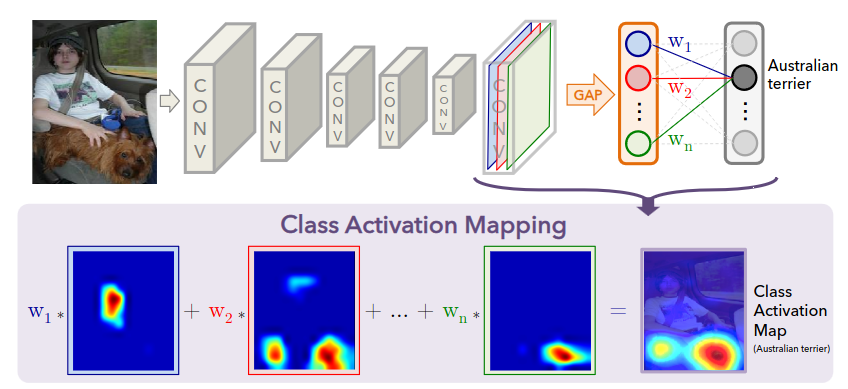
\includegraphics[width=3.25in]{figure/cam.png}}
\caption{Figure taken from \cite{cam}, showing the steps required to create a Class Activation Map}
\label{camimg}
\end{figure}

Although CAM is an intuitive and effective method of visualizing the inner workings of a CNN, it has some downsides. Firstly, it is highly model dependent, requiring that the model only have a single dense layer after the convolutions. Although there are some state of the art models which only use a single dense layer, this still places a limit on what models can be used, or requires the simplification of models that use more than a single dense layer. \cite[4]{cam} notes a 1-2\% drop in classification performance when performing this simplification. Secondly, the output of CAM is simply a weighted sum of all the feature maps after the final convolutional layer. As we move deeper in a CNN, we reduce the spatial resolution by downsampling, while increasing the number of channels (increasing the depth of the output while reducing the height and width). Because of this, the CAM will have a drastically lower resolution than the original image, often less than $10 x 10$ while the input image may be hundreds of pixels in both dimensions. Because of this, CAM can only show general areas, as opposed to pixel wise explanations.
\\

\subsubsection{Gradient Class Activation Mapping (Grad-CAM)}

Grad-CAM \cite{gradcam} is an improvement on CAM, which generalizes the method to function with any CNN architecture, thus making the method much less model dependent and avoiding the performance drop incurred when simplifying the model with CAM. Instead of using the weights of a final layer to calculate a weighted sum of feature maps in the last convolutional layer, Grad-CAM uses gradients flowing from the relevant output node to the activation maps to calculate the weights for each feature map. Furthermore, the authors prove that this method is a strict generalization of CAM \cite[5]{gradcam}, so that no information is lost by using gradients instead of weights.

Like the simplicity of the CAM method, the calculation of the weights using the gradients is also quite simple, as seen in Equation \ref{gradcameq}.

\begin{equation}
\alpha^c_k = \frac{1}{Z} \sum_i \sum_j \frac{\delta y^c}{\delta A^k_{ij}}
\label{gradcameq}
\end{equation}

Here, $c$ represents the index of the class we are interested in, $k$ the index of the feature map, and $i$ and $j$ the width and height of the image. $y^c$ is the element of the output vector $y$ which corresponds to the class $c$, while $A^k$ is the $k$'th feature map. $Z$ is equal to $i * j$, and simply normalizes the sum. Thus, we are actually just performing global average pooling of the gradients of $A^k$ with respect to $y^c$, which gives us a single value we can use as the weight for this feature map. Doing this for all feature maps for a specific class gives us all the weights we need to calculate a weighted sum, which we can upsample and visualize to get an explanation for the decision of the CNN.
\\

\subsubsection{Guided Backpropagation}

\subsubsection{Layer-Wise Relevance Propagation (LRP)}

LRP is another XAI method which generates a visual explanation of the areas of an image which lead to a classification decision. Unlike CAM and Grad-CAM, LRP outputs a map which describes the relevance of every single pixel in the input image, and is thus produces a much more fine grained explanation than these other methods. LRP also differs in that \cite{lrp} does not define it as a specific method, but rather as a concept defined by a certain set of constraints which can be satisfied by different implementations depending on the type of model.

LRP assumes that we can model the relevance $R_i$ for any node $i$ in a neural network, and aims to find the relevance for all the input nodes (the pixels in an image). Relevance is the contribution of any node to the final prediction $f(x)$ of a network, and the idea is to take the relevance of the output layer (simply defined as the output $f(x)$), and iteratively propagate this backwards through the network. Relevance scores are subject to a conservation property, which means that the sum of relevances must be equal for all layers (Equation \ref{lrpeq}). Furthermore, nodes must also conserve relevance, such that the sum of relevances a node receives from the previous layer is equal to the amount it distributes to the next layer. Once the relevance scores have been propagated from the output to the input layer in accordance with these constraints, we have a measure for how each input pixel contributed to the final output.

\begin{equation}
f(x) = ... = \sum_{d \in l + 1} R^{(l + 1)}_d = \sum_{d \in l + 1} R^{(l + 1)}_d = ... = \sum_d R^{(1)}_d
\label{lrpeq}
\end{equation}

To distribute relevance between the nodes in a way which obeys the constraints defined in Equation \ref{lrpeq}, a rule for propagation of relevances must be defined. As \cite{lrp} shows, simply satisfying the constraints is not guaranteed to lead to meaningful explanations, nor is the decomposition of relevance unique. However, they show that by using a suitable propagation rule, we gain a visual explanation which shows which areas contribute to the final decision and which areas make the final decision less likely \cite[28]{lrp}.

\section{Out-of-Distribution Detection}

\bibliographystyle{apalike}
\bibliography{bibliography}


\end{document}
